\chapter{Large-scale datasets for Switzerland}
\label{data}

% SOURCE: PV paper (original draft)
% Using big data mining techniques for the estimation of large-scale RPV potential requires the availability of accurate and high-resolution environmental and building datasets. Spatial and temporal resolutions of these data are rapidly increasing, but the highest-quality information is frequently not available for a large spatial coverage. Switzerland has been selected as case study area for this approach, as large amounts of data at different resolutions and spatial coverage exist for solar radiation, the building stock and digital surface models.

The spatio-temporal modelling of solar photovoltaic and shallow geothermal energy potentials at national scale for Switzerland requires the availability of high-resolution data on the existing building stock, meteorological data and data on the subsurface geology. 
As most of these data are used several times throughout this work and may play an important role in the choice of suitable modelling approaches, the relevant large-scale datasets used throughout this thesis and relevant pre-processing steps are detailed in the following.

\section{Building and landscape data}
A large amount and variety of building and landscape data is available for Switzerland. These include statistics related to the existing building stock and their use for the residential and service sector, the geometries of building footprints, rooftops and other built-up areas, as well as high-resolution digital elevation models. Most of this data can be accessed freely on the mapping platform of the Swiss Confederation\footnote{\url{https://map.geo.admin.ch/}}.  Table~\ref{tab:bld_landscape} shows an overview of all building and landscape data used throughout this thesis, with a short explanation of each of the datasets provided below.

\begin{table}[tb]
\centering
\footnotesize
\caption{Overview of building and landscape datasets and the relevant chapters where the data is used. \textit{CH}: Entire Switzerland, \textit{GE, LU}: Cantons of Geneva and Luzern.}
\label{tab:bld_landscape}
\resizebox{\textwidth}{!}{%
\begin{tabular}{lllllll}
\hline
\textbf{Type}                                   & \textbf{Dataset}     & \textbf{Coverage} & \textbf{Spatial res.} & \textbf{Creation} & \textbf{Source} & \textbf{Chapter} \\ \hline
\multirow{2}{*}{\textit{Statistics}}                     & RBD                  & CH                & Building                    & 2015/2019         & FSO \cite{bundesamt_fur_statistik_bfs_eidgenossisches_2015}            & \ref{solar},\ref{hybrid_chapter}         \\
                                                & STATENT              & CH                & $100 \times 100 m^2$        & 2018              & FSO \cite{bfs_statistik_2018}            & \ref{hybrid_chapter}               \\ \hline
\multirow{5}{*}{\begin{tabular}[c]{@{}l@{}}\textit{Building /} \\ \textit{landscape} \\ \textit{geometries}\end{tabular}} & Building footprints  & CH             & Building                    & 2017              & swisstopo  \cite{swisstopo_swisstlm3d_2018}       & \ref{solar},\ref{geothermal}, \ref{hybrid_chapter}    \\
                                                & Building parcels     & CH (ex. LU)       & Parcel                      & various           & Cantons*        & \ref{geothermal}, \ref{hybrid_chapter}    \\
                                                & Roof surfaces        & CH                & Rooftop                     & 2010-2016      & Sonnendach.ch   \cite{klauser_solarpotentialanalyse_2016}       & \ref{solar},\ref{hybrid_chapter}      \\
                                                & Roof superstructures & GE                & Rooftop                     & 2005-2011  & SITG  \cite{sitg_superstructures_2019}          & \ref{solar}                \\
                                                & TLM                  & CH                & various                     & 2017              & swisstopo \cite{swisstopo_swisstlm3d_2018}      & \ref{geothermal}           \\ \hline
\multirow{3}{*}{\begin{tabular}[c]{@{}l@{}}\textit{Digital} \\ \textit{elevation} \\ \textit{models}\end{tabular}}       & DTM                  & CH                & $2 \times 2 m^2$            & 2010-2016         & swisstopo  \cite{swisstopo_swissalti3d_2017}     &\ref{solar}             \\
                                                & DSM                  & CH                & $2 \times 2 m^2$            & 2000-2008         & swisstopo   \cite{swisstopo_dsm_2005}    & \ref{solar}                \\
                                                & DSM                  & GE                & $0.5 \times 0.5 m^2$        & 2013              & SITG  \cite{sitg_mns_2018}          & \ref{solar}   \\ \hline
\multicolumn{7}{l}{* Data has been collected from individual cantonal offices for all cantons except Luzern (see Appendix \ref{app:canton_parcels})}                                           
\end{tabular}%
}
\end{table}

\subsection{Building and enterprise statistics}
\label{data_rbd_statent}
\textbf{Registry of Buildings and Dwellings (RBD).} The RBD, published and continously updated by the Swiss Federal Statistical Office (FSO) \cite{bundesamt_fur_statistik_bfs_eidgenossisches_2015}, contains 2.2 million registered buildings in Switzerland.
It lists a large amount of building-related attributes, including building coordinates, floor area, construction period, number of floors, number of dwellings, and information on the building use (e.g. residential/service sector/industrial). 
The RBD further contains a registry of 4.6 million dwellings, amongst other listing the dwelling's area, number of rooms and dwelling use.
\nomenclature[A]{RBD}{Registry of Buildings and Dwellings}
As the attributes in the RBD are missing for some buildings and dwellings, we estimate the missing characteristics in order to estimate RE potentials for the entire building stock. Details for the pre-processing steps to fill missing data are described in Appendix \ref{app:rbd}.

\textbf{Structural Business Statistic (STATENT).} In addition to the RBD, the STATENT provides information on the number of enterprises and employees in each of the service and industrial sectors, at a resolution of $100 \times 100 m^2$ pixels for Switzerland \cite{bfs_statistik_2018}. The sectors are divided according to the Swiss General Classification of Economic Activities (NOGA) into 88 NOGA codes \cite{bfs_noga_2008}, which we group to 19 sub-sectors as described in Appendix \ref{app:noga}.
\nomenclature[A]{STATENT}{Structural Business Statistic}
\nomenclature[A]{NOGA}{General Classification of Economic Activities}

\subsection{Building and landscape geometries}
\label{data_geometry}

\textbf{Building footprints.} 
Geometries of the building footprints for the entire Swiss building stock are available as 3.7 million vector polygons. 
The polygons are part of the Topographic Landscape Model (TLM) of Switzerland published by the Swiss Federal Office of Topography (swisstopo) \cite{swisstopo_swisstlm3d_2018}. 
The footprints are based on a 3D model of the Swiss building stock, which is created using a photogrammetric capturing method and has a high precision of $\pm 0.3 m$.
% SOURCE: PV paper (original draft)
% We compute the RPV potential per roof surface, based on a national-scale dataset of building rooftops.
\nomenclature[A]{TLM}{Topographic Landscape Model}
%\nomenclature[A]{swisstopo}{Swiss Federal Office of Topography}

\textbf{Parcel geometries.}
In contrast to the building footprints, information on the boundaries of property units (parcels) are not collected at national level for Switzerland. 
Parcel geometries, which are vector polygons derived from official mensuration data, are instead available from cantonal geoinformation services. 
As parcel data provides valuable insights in the attribution of surrounding land to building footprints, we have collected parcel geometry data for 25 of the 26 Swiss cantons separately.
In most cantons, this data is entirely available, while some areas are missing for a small number of cantons (see Appendix \ref{app:canton_parcels} for an overview of the data sources and availability). Only for the canton of Luzern no parcel data was obtained.
% The parcel boundaries are vector representations of the official mensuration data for around 100,000 property units, obtained from the cantonal geoinformation services of Vaud (ASIT-VD) \cite{asit_vd_cadastre_2019} and Geneva (SITG) \cite{sitg_parcelles_2020}.
%\nomenclature[A]{ASIT-VD}{Geoinformation service (Vaud)}
%\nomenclature[A]{SITG}{Geoinformation service (Geneva)}

\textbf{Roof surfaces.}
This dataset contains 9.6 million vector polygons which are derived from a national 3D building model (LOD~2) by swisstopo \cite{klauser_solarpotentialanalyse_2016}.
The roof polygons represent the roofs of the 3.7 million building footprints in Switzerland and contain information  on the tilt, aspect and tilted area of each roof.
This data has has been published as part of a previous study of RPV potential in the Switzerland, carried out by the Swiss Federal Office of Energy (SFOE), titled and referred to throughout this thesis as "Sonnendach.ch" \cite{klauser_solarpotentialanalyse_2016}.
%\nomenclature[A]{SFOE}{Swiss Federal Office of Energy}

\textbf{Roof superstructures.}
In the Canton of Geneva, where detailed city GML data (LOD~4) exists, an additional dataset of roof superstructures is available through SITG~\cite{sitg_superstructures_2019}. %NEED TO ADD SOURCE
These superstructures are vector polygons which represent objects on rooftops such as dormers and chimneys. 
Furthermore, small roof shapes such as dormers, which are generally unsuitable for installing PV, are partly represented as separate roof polygons in the LOD~4 dataset.
For this reason, we convert all surfaces smaller than $8m^2$ are converted to superstructures. 
As the superstructure dataset has been derived from LiDAR data, building-integrated objects such as windows or already existing solar panels are not considered. 
Furthermore, roofs without any superstructure information are excluded from the analysis, as a visual inspection showed that this data is missing on a large part of the rooftops. Using only rooftops where superstructure information is available yields a dataset of 37.7K roofs in the Canton of Geneva. 

\textbf{Topographic Landscape Model (TLM).}
In addition to the building footprints, the TLM \cite{swisstopo_swisstlm3d_2018} and contains a detailed 3D representation of various landscape objects in vector form. 
These include built-up areas (e.g. roads, railways, parking lots, sports facilities etc.), natural (e.g. lakes, rivers) and artificial (e.g. pools) water bodies and land cover data (e.g. forests, wetlands, agricultural use, glaciers), protected areas, and more
\footnote{See \url{https://www.swisstopo.admin.ch/en/geodata/landscape/tlm3d.html} for a full list of attributes}.
The TLM has a precision of $0.2-1.5m$ for well-defined objects such as roads or buildings, and of $1 - 3m$ for other landscape features such as forests \cite{swisstopo_swisstlm3d_2018}. 
To create a homogeneous dataset of vector polygons, relevant line data, namely roads and railways, are buffered (expanded) by their width (see Appendix \ref{app:roads}).
Other TLM objects used in Chapter \ref{geothermal} are buffered by $1m$ to account for the imprecision of the TLM.

\subsection{Digital Elevation models}
\label{data_DEM}
\textbf{Digital Terrain Model.} Two types of surface datasets are used for the estimation of PV potential: A Digital Terrain Model (DTM) and a Digital Surface Model (DSM) of Switzerland. The DTM is a high-resolution surface model, without considering vegetation and constructions. It is available at national scale as pixels of $2\times2$ m$^2$ resolution. The DTM is derived from Light Detection and Ranging (LiDaR) data that was collected in the period from 2000-2008 and has been updated from 2010-2016.
%
It contains information on coordinates (x,y) and altitude (z). In addition, we consider several spatial features derived from the DTM at various spatial scales, including terrain slope and curvature (see Table \ref{tab:DTM_ftrs} for a complete list). These features have been computed by \citet{robert_spatial_2012} for an aggregation level of $250 \times 250$ m$^2$.

\begin{table}[b]
\centering
\footnotesize
\caption{Spatial features of the DTM (x,y,z) and additional features derived from the DTM. All derived features are available for each scale~\cite{robert_spatial_2012}.}
\label{tab:DTM_ftrs}
\begin{tabular}{cll}
\hline
\textbf{Coordinates} & \textbf{Derived features} & \textbf{Scales} \\ \hline
x                    & slope                           & 250m (small)    \\
y                    & directional slope (NS, EW)      & 1.75km (med)    \\
z                    & curvature (DoG)                 & 3.75km (big)    \\ \hline
\end{tabular}
\end{table}

\textbf{Digital Surface Model.} The DSM is a complete model of the landscape, including all visible landscape elements. As the DTM it is available  in $2\times2$ m$^2$ resolution from LiDaR data that was collected in the period from 2000-2008, but contrary to the DSM is has not been updated. More recent DSMs have however been created for individual cantons in Switzerland at a resolution of $0.5\times0.5$ m$^2$. 
%
We use the higher-resolution and more updated DSM for the canton of Geneva to improve the estimation of RPV potential.
This has two-fold reasons. Firstly, the spatial resolution of the updated DSM is 16 times higher, and secondly, the newer period of construction accounts for some buildings which have been built after the completion of the first DSM.
An analysis of the RBD shows that 9.32\% of buildings in Switzerland have been constructed in the period of 2006-2015, corresponding approximately to the time span between the two studies. In Geneva, this fraction is comparable (7.28\%).

\nomenclature[A]{DTM}{Digital Terrain Model}
\nomenclature[A]{DSM}{Digital Surface Model}
\nomenclature[A]{LiDaR}{Light Detection and Ranging}

\section{Meteorological data}
\label{data_meteo}
Meteorological data is available from the Swiss Federal Office of Meteorology and Climatology (MeteoSwiss) as gridded data and for a network of measurement stations across the country. 
Gridded data is preferred over data from measurement stations as it provides a better spatial coverage with an increased spatial resolution and has a very low missing data ratio ($<1\%$). 
For the potential studies in Part~\ref{potential}, we use solar radiation and temperature data for Switzerland. We further derive heating and cooling degree days (HDD/CDD), which are used to estimate monthly variations of heating and cooling demands \cite{stadler_contribution_2018}. The meteorological datasets are summarised in Table~\ref{tab:meteo}.
%\nomenclature[A]{MeteoSwiss}{Swiss Federal Office of Energy}
\nomenclature[A]{HDD}{Heating Degree Days}
\nomenclature[A]{CDD}{Cooling Degree Days}

\begin{table}[b]
\centering
\footnotesize
\caption{Overview of meteorolgical datasets and the relevant chapters. }
\label{tab:meteo}

\begin{tabular}{lllllll}
\hline
\textbf{Type}                    & \textbf{Dataset}            & \textbf{Spatial res.} & \textbf{Time} & \textbf{Range} & \textbf{Source} & \textbf{Chapter}   \\ \hline
\multirow{3}{*}{\begin{tabular}[c]{@{}l@{}}\textit{Solar} \\ \textit{radiation}\end{tabular}} & GHI & $1.25$ deg. min.*   & hourly        & 2004-2015      & MeteoSwiss \cite{stockli_daily_2013}     & \ref{solar}              \\
                                 & DIR & $1.25$ deg. min.*   & hourly        & 2004-2015      & MeteoSwiss  \cite{stockli_daily_2013}    & \ref{solar}              \\
                                 & Albedo              & $1.25$ deg. min.*   & hourly        & 2004-2015      & MeteoSwiss \cite{stockli_daily_2013}     & \ref{solar}              \\ \hline
\multirow{3}{*}{\textit{Temperature}}     & Max. temp.   & $1 \times 1$ km$^2$    & daily         & 2004-2015      & MeteoSwiss \cite{meteoswiss_daily_2017}     & \ref{solar}              \\
                                 & HDD                 & $200 \times 200$ m$^2$  & daily         & averaged      & Eq.~\ref{eq:hdd}     & \ref{geothermal}, \ref{hybrid_chapter} \\
                                 & CDD                 & $200 \times 200$ m$^2$  & daily         & averaged      & Eq.~\ref{eq:cdd}    & \ref{geothermal}         \\ \hline
\multicolumn{7}{l}{* Deg. min.: degree minutes on a longitude-latitude grid (1.25 deg. min. $\approx 1.6 \times 2.3$ km$^2$)}   
\end{tabular}
\end{table}


\subsection{Solar radiation}
\label{data_solarRad}

% SOURCE: PV paper (original draft)
\textbf{Global and direct horizontal radiatio (GHI/DIR).} To estimate RPV potential, we use satellite data for global horizontal radiation (GHI), also known as surface incoming shortwave radiation, and direct beam radiation (DIR) provided by MeteoSwiss\cite{stockli_daily_2013}. The radiation describes the  solar power at the earth's surface, given in W/m$^2$. The solar energy is called irradiation, given in Wh/m$^2$. The data are hourly values for the period from 2004-2015 on a longitude-latitude grid of 1.25 degree minutes, equivalent to around $1.6 \times 2.3$ km$^2$ (see Fig.~\ref{figa:GHI_patterns}).  
\nomenclature[A]{GHI}{Global horizontal radiation}
\nomenclature[A]{DIR}{Direct beam radiation}

We average the 12 years of satellite data in order to obtain an average year in hourly resolution, i.e. $12 \times 365$ time steps for 11,243 satellite pixels (see Fig.~\ref{figb:GHI_patterns}). This reduces the variability of the radiation data, and allows the estimation of long-term RPV potential without bias due to extreme meteorological events of a specific year. Furthermore, all hours with constantly zero GHI measurements are removed (i.e. night hours). The remaining 10-17 day hours result in $\sim~3-6$ million hourly values for GHI and DIR per month, depending on the month. 

\textbf{Surface albedo.} A dataset for surface reflectance, also referred to as surface albedo, is available at the same spatio-temporal resolution as the global and direct horizontal radiation. In particular in Switzerland, where a large part of the country is covered by mountains, the surface albedo plays an important role in the quantification of the reflected solar radiation component \cite{kahl_bright_2019}. As the surface albedo shows low variations throughout the day, the data is aggregated to daily values, before being averaged across the 12 years as described above. 

All solar radiation data has been derived by MeteoSwiss from Meteosat Second Generation (MSG) satellite observations using the Heliomont algorithm~\cite{stockli_heliomont_2017}. It was developed to improve the quality of the results, particularly in Switzerland's Alpine territories. 
\citet{ineichen_long_2014} performed a comprehensive validation of various satellite-based products against measurement data, and found a negligible bias of the hourly satellite data across 18 measurement stations. 
The standard deviation for hourly global and direct radiation is 19\% and 39\%, respectively.

\begin{figure}[tb]
\centering
\begin{subfigure}{.49\textwidth}
  \centering
  % include second image
  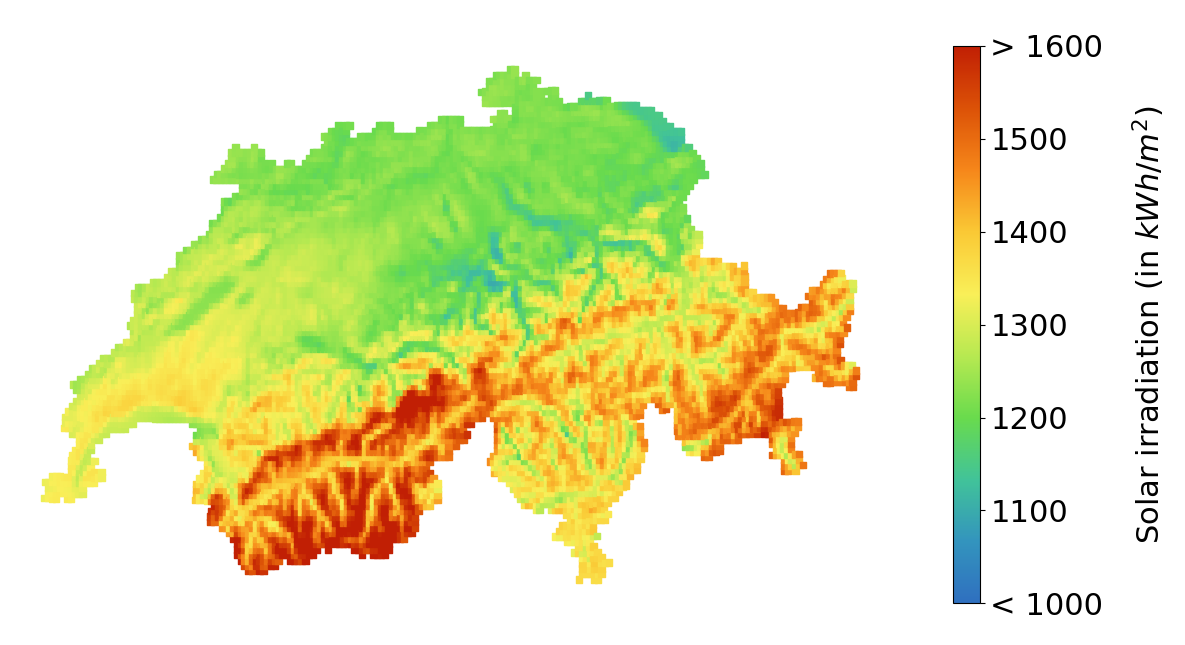
\includegraphics[width=\linewidth]{Figs/yr_raw.png}  
  \caption{}
  \label{figa:GHI_patterns}
\end{subfigure}
\begin{subfigure}{.49\textwidth}
  \centering
  % include first image
  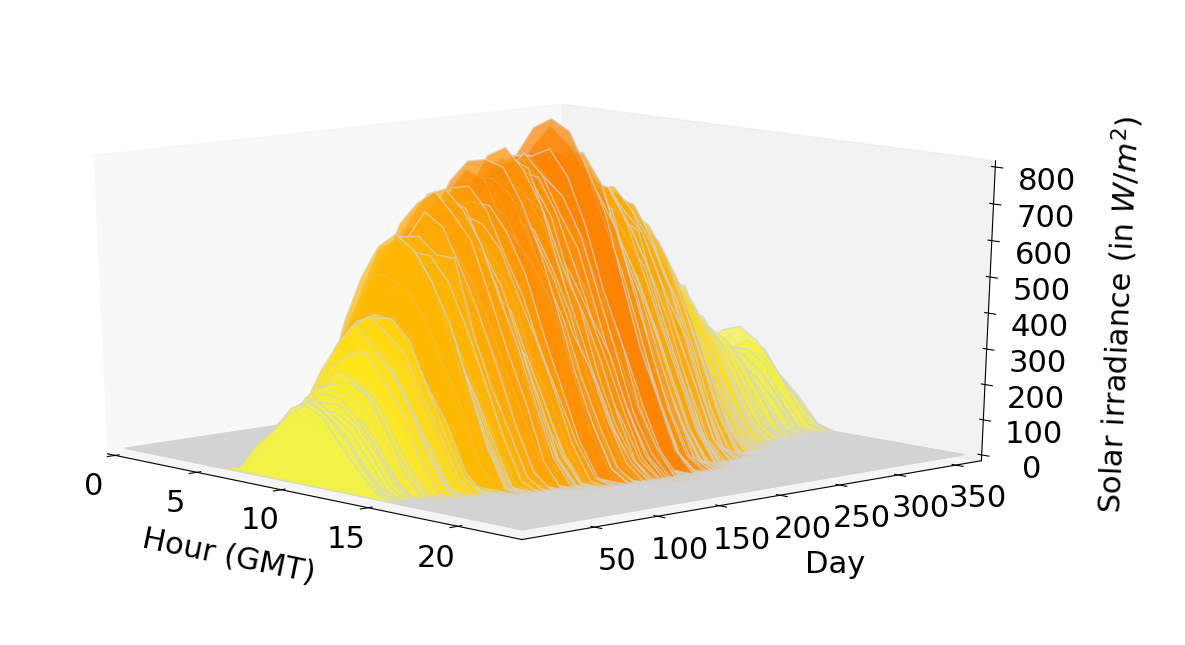
\includegraphics[width=\linewidth]{Figs/hours.png}  
  \caption{}
  \label{figb:GHI_patterns}
\end{subfigure}
\caption{(a) Yearly solar irradiation ($G_h$) satellite data, (b) hourly $G_h$ at selected location (mean of 2004-2015).}
\label{fig:GHI_patterns}
\end{figure}

\subsection{Temperature}

\textbf{Maximum daily air temperature.} Air temperature data, including the daily mean, maximum and minimum air temperature, is available from MeteoSwiss on a grid of $1 \times 1$ km$^2$ for Switzerland \cite{meteoswiss_daily_2017}. 
In contrast to the solar radiation, MeteoSwiss uses near-surface air temperature measurements from meteorological stations, which are interpolated in three dimensions, with further adjustments to account for temperatures in high mountain areas \cite{meteoswiss_daily_2017}.
For coherence with the solar radiation data described above, we collect daily air temperature data for the years of $2004-2015$. 
We use maximum air temperature in the estimation of RPV potential (Chapter~\ref{solar}) as the maximum solar yield occurs around midday when temperatures are near their daily maximum, resulting in a conservative estimate of the PV panel efficiency.

\textbf{Heating degree days (HDD).}
\label{app:HDD}
The HDD is defined in the norm SIA 2028 as the sum of the heating degrees for each month $m$, averaged across 20 years, such that \cite{sia_klimadaten_2010}: 
\begin{equation}
\label{eq:hdd}
    HDD = \frac{1}{20} \sum_{y=1}^{20} \sum_{d=1}^{d_m} (20 - T_{m}(d, m, y)) \quad \forall T_{m} (d, m, y) \leq 12 ^\circ C. 
\end{equation}

where $d_m$ is the number of days of each month and $T_{m}$ is the daily mean temperature on day $d$ in month $m$ of year $y$. 
We use gridded daily mean air temperature data for 20 years ($1991-2011$) \cite{meteoswiss_daily_2017} to compute the HDD for each of the $1 \times 1$  km$^2$ pixels of the temperature grid (see above). The time span of  $1991-2011$ is chosen such as to yield results that are comparable to the tabulated HDD in \cite{sia_klimadaten_2010}.
The HDD is then spatially interpolated to a resolution of $200 \times 200$ m$^2$ using a Random Forest algorithm (see Section \ref{RF}) with the pixel coordinates and the altitude (obtained from DTM) as features.

\textbf{Cooling degree days (CDD).} In contrast to the HDD, no Swiss norm exists for the computation of CDD. We hence obtain the CDD from \cite{christenson_climate_2006} using a reference temperature of $18 ^\circ C$:
\begin{equation}
\label{eq:cdd}
    CDD = \frac{1}{20} \sum_{y=1}^{20} \sum_{d=1}^{d_m} (T_{m}(d, m, y)-18) \quad \forall T_{m} (d, m, y) \geq 18 ^\circ C. 
\end{equation}
for the same timespan ($1991-2011$) and spatial resolution ($1 \times 1$ km$^2$) as the HDD, which is then interpolated to pixels of $200 \times 200$ m$^2$ as described above.

\section{Subsurface data [\textit{PRELIMINARY}]}
\label{data_geo}

Subsurface data are more scarcely available than building or meteorological data. 
The available subsurface data include national maps of the geological characteristics of the Swiss terrain, digitalised by swisstopo, as well as cantonal geothermal cadastres containing maps of the thermal ground properties. 
These geothermal cadastres with high-resolution data of the thermal ground properties can be obtained for the Cantons of Vaud (provided by ASIT-VD \cite{asit_vd_cadastre_2019-1}) and Geneva (provided by SITG \cite{sitg_cadastre_2019}). 
In addition, the cadastres contain information on restriction zones for geothermal installations within the case study area and existing installations.
At national scale, this information is complemented by national data regarding protected areas and groundwater vulnerability to assess restrictions for geothermal installations.
% Furthermore, information on restrictions for geothermal installations can be obtained from cantonal geothermal cadastres and national information regarding protected areas and groundwater vulnerability. 
An overview of the datasets described below is provided in Table~\ref{tab:geoData}.

\begin{table}[b]
\centering
\footnotesize
\caption{Overview of subsurface datasets. CH denotes availablility in the entire Switzerland, VD is the Canton of Vaud and GE is the Canton of Geneva.}
\label{tab:geoData}
\resizebox{\textwidth}{!}{%
\begin{tabular}{llllll}
\hline
\textbf{Type} & \textbf{Dataset} & \textbf{Coverage} & \textbf{Spatial res.} & \textbf{Source} & \textbf{Chapter} \\ \hline
\multirow{3}{*}{\textit{\begin{tabular}[c]{@{}l@{}}Geological  \\ characteristics\end{tabular}}} & GK500 Lithology types & CH & Polygons & swisstopo \cite{swisstopo_geomaps_nodate} & \ref{geothermal} \\
 & \begin{tabular}[c]{@{}l@{}}Thickness of \\ unconsolidated rocks\end{tabular} & CH (partly) & $25 \times 25$ m$^2$ & swisstopo & \ref{geothermal} \\ \hline
\multirow{3}{*}{\textit{\begin{tabular}[c]{@{}l@{}}Thermal \\ ground\\ properties\end{tabular}}} & Thermal conductivity ($\lambda$) & VD,GE & $50 \times 50 \times 50$ m$^3$ & ASIT-VD \cite{asit_vd_cadastre_2019-1}, SITG \cite{sitg_cadastre_2019} & \ref{geothermal} \\
 & Heat capacity ($\rho C$) & VD,GE & $50 \times 50 \times 50$ m$^3$ & SITG \cite{sitg_cadastre_2019} & \ref{geothermal} \\
 & Surface   temperature ($T_0$) & CH & $200 \times 200$ m$^2$ & \citet{assouline_machine_2019} & \ref{geothermal} \\\hline
\multirow{3}{*}{\textit{\begin{tabular}[c]{@{}l@{}}Installation   \\ restrictions\end{tabular}}} & Restriction zones & VD, GE & Polygons & ASID-VD \cite{asit_vd_cadastre_2019-1}, SITG \cite{sitg_cadastre_2019} & \ref{geothermal} \\
 & Groundwater vulnerability & CH & Polygons & swisstopo \cite{swisstopo_geomaps_nodate} & \ref{geothermal} \\
 & Protected zones & CH & Polygons & swisstopo \cite{swisstopo_swisstlm3d_2018} & \ref{geothermal} \\ \hline
\end{tabular}
}
\end{table}

\subsection{Geological characteristics}

\begin{figure}[tb]
\centering
\begin{subfigure}{.49\textwidth}
  \centering
  % include second image
  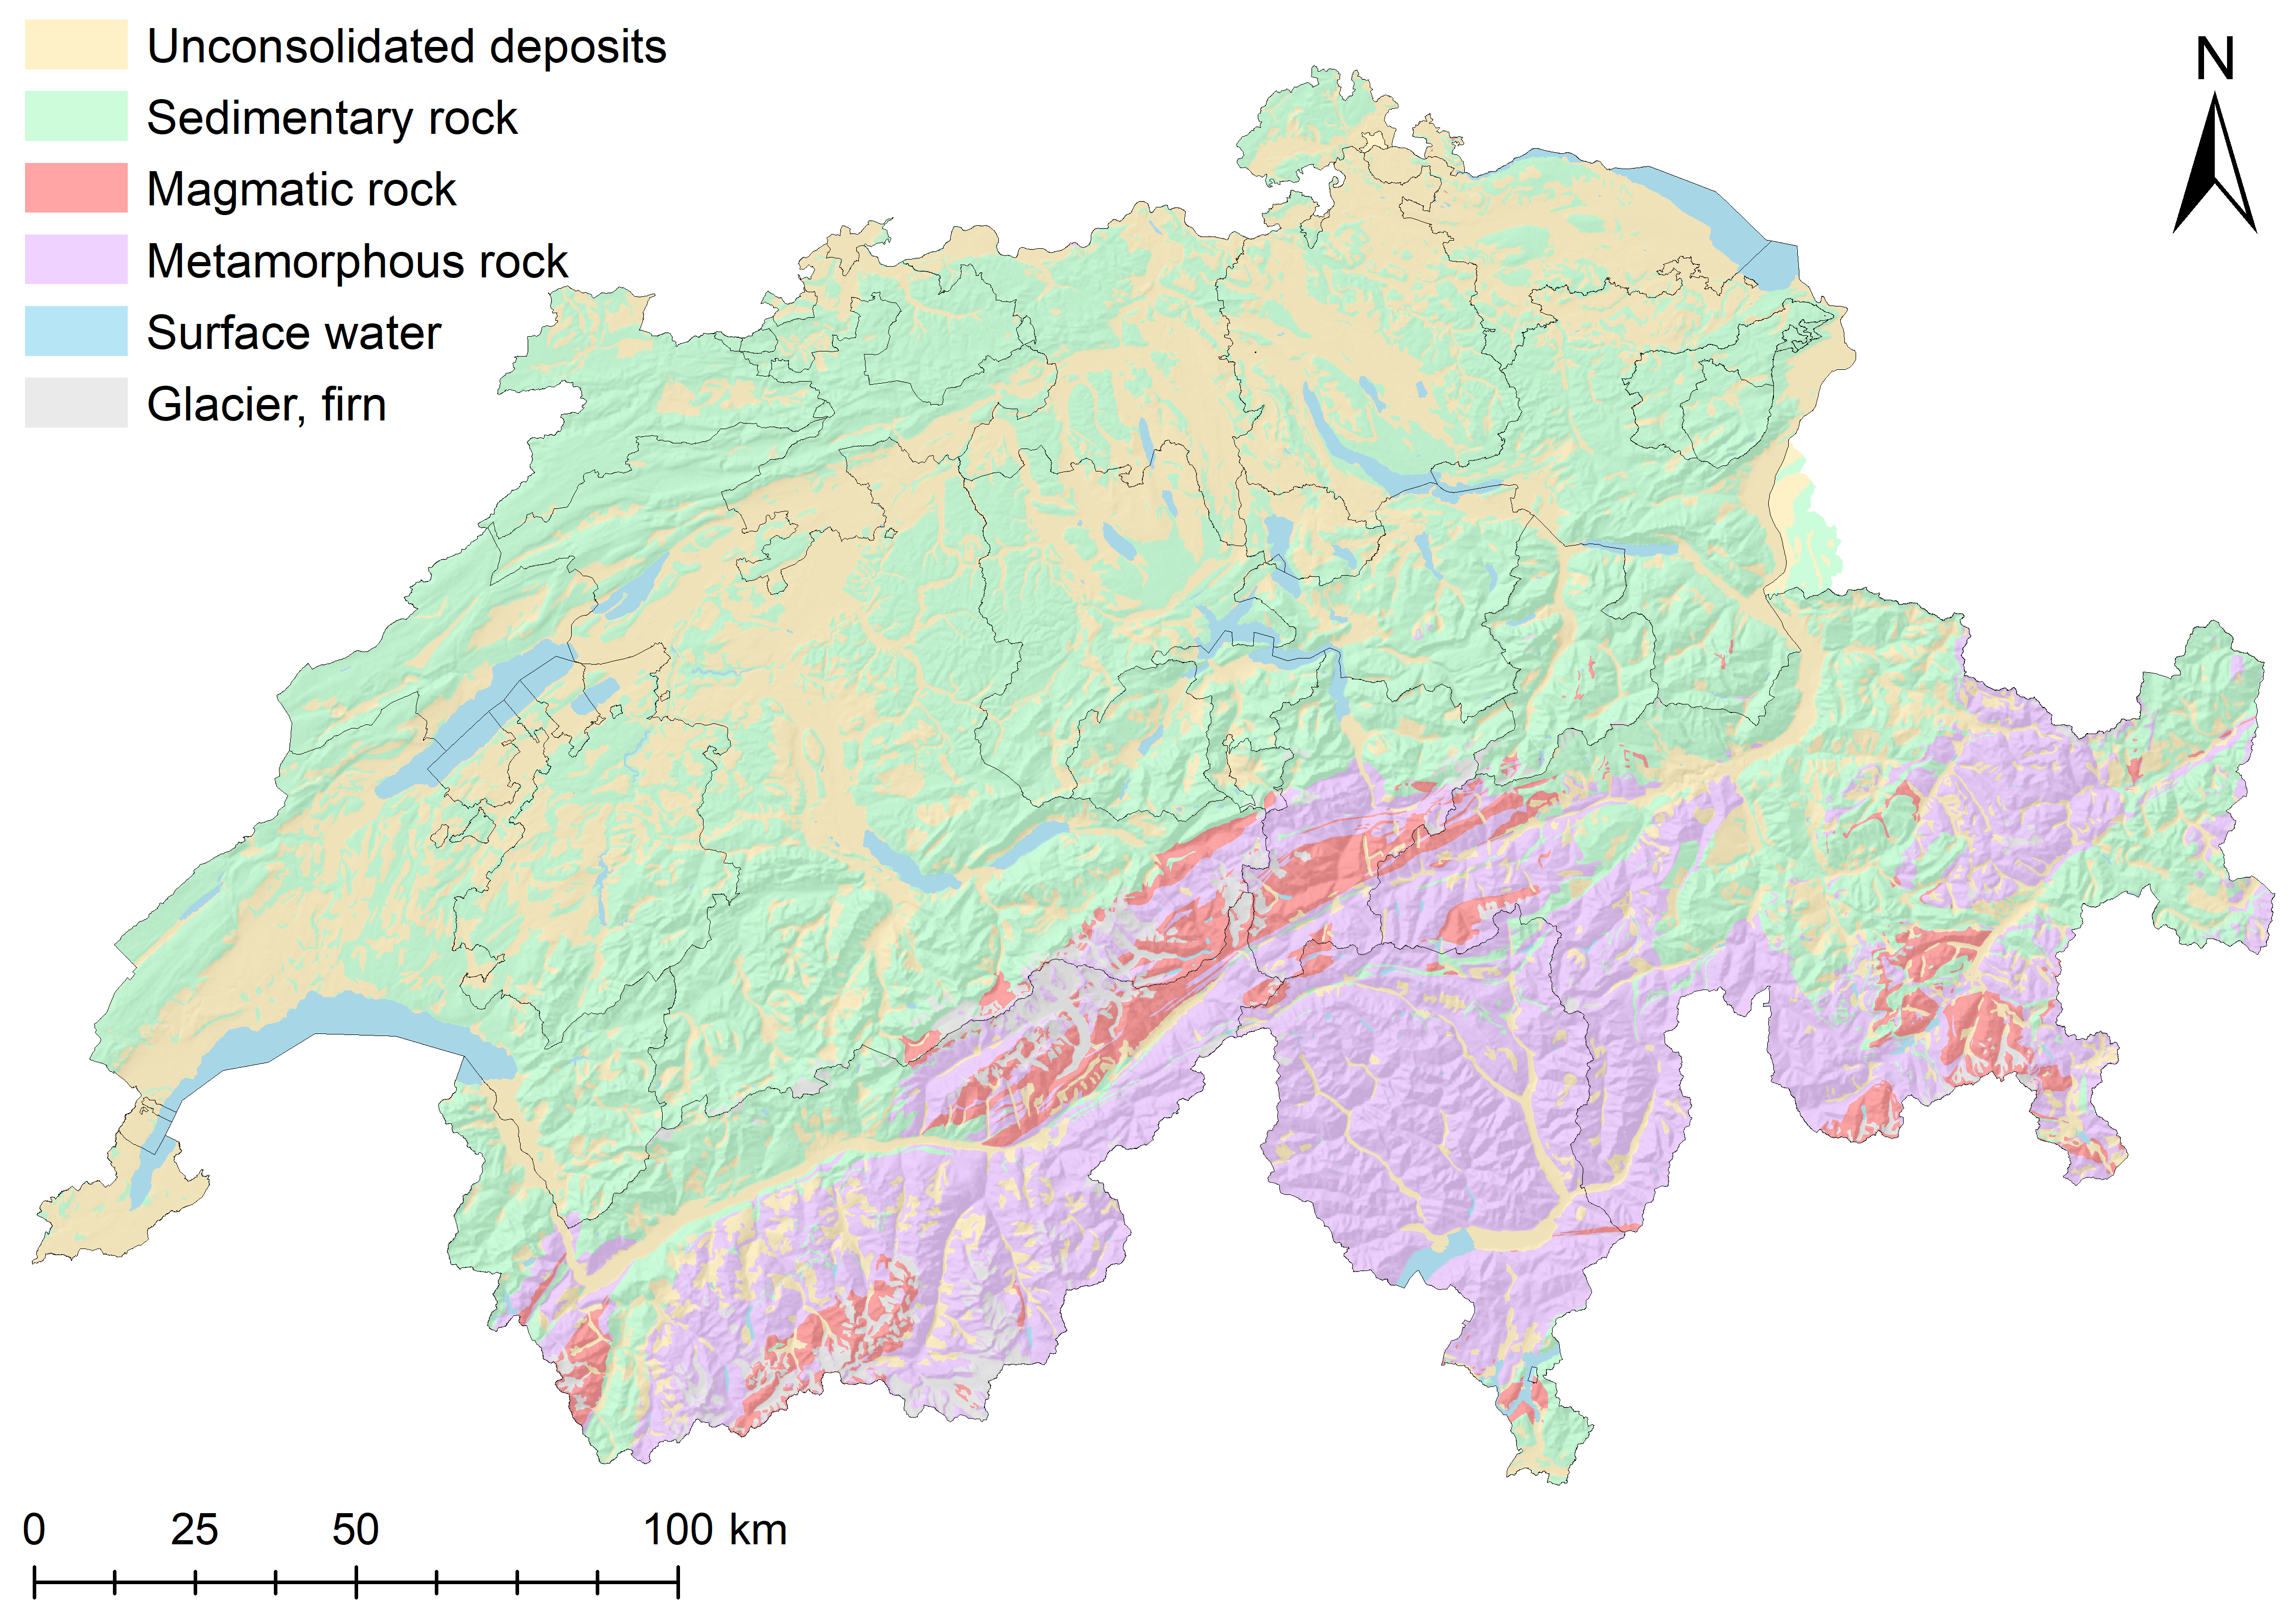
\includegraphics[width=.9\linewidth]{images/Figs/rockType_CH.png}  
  \caption{}
  \label{figa:geoCH}
\end{subfigure}
\begin{subfigure}{.49\textwidth}
  \centering
  % include first image
  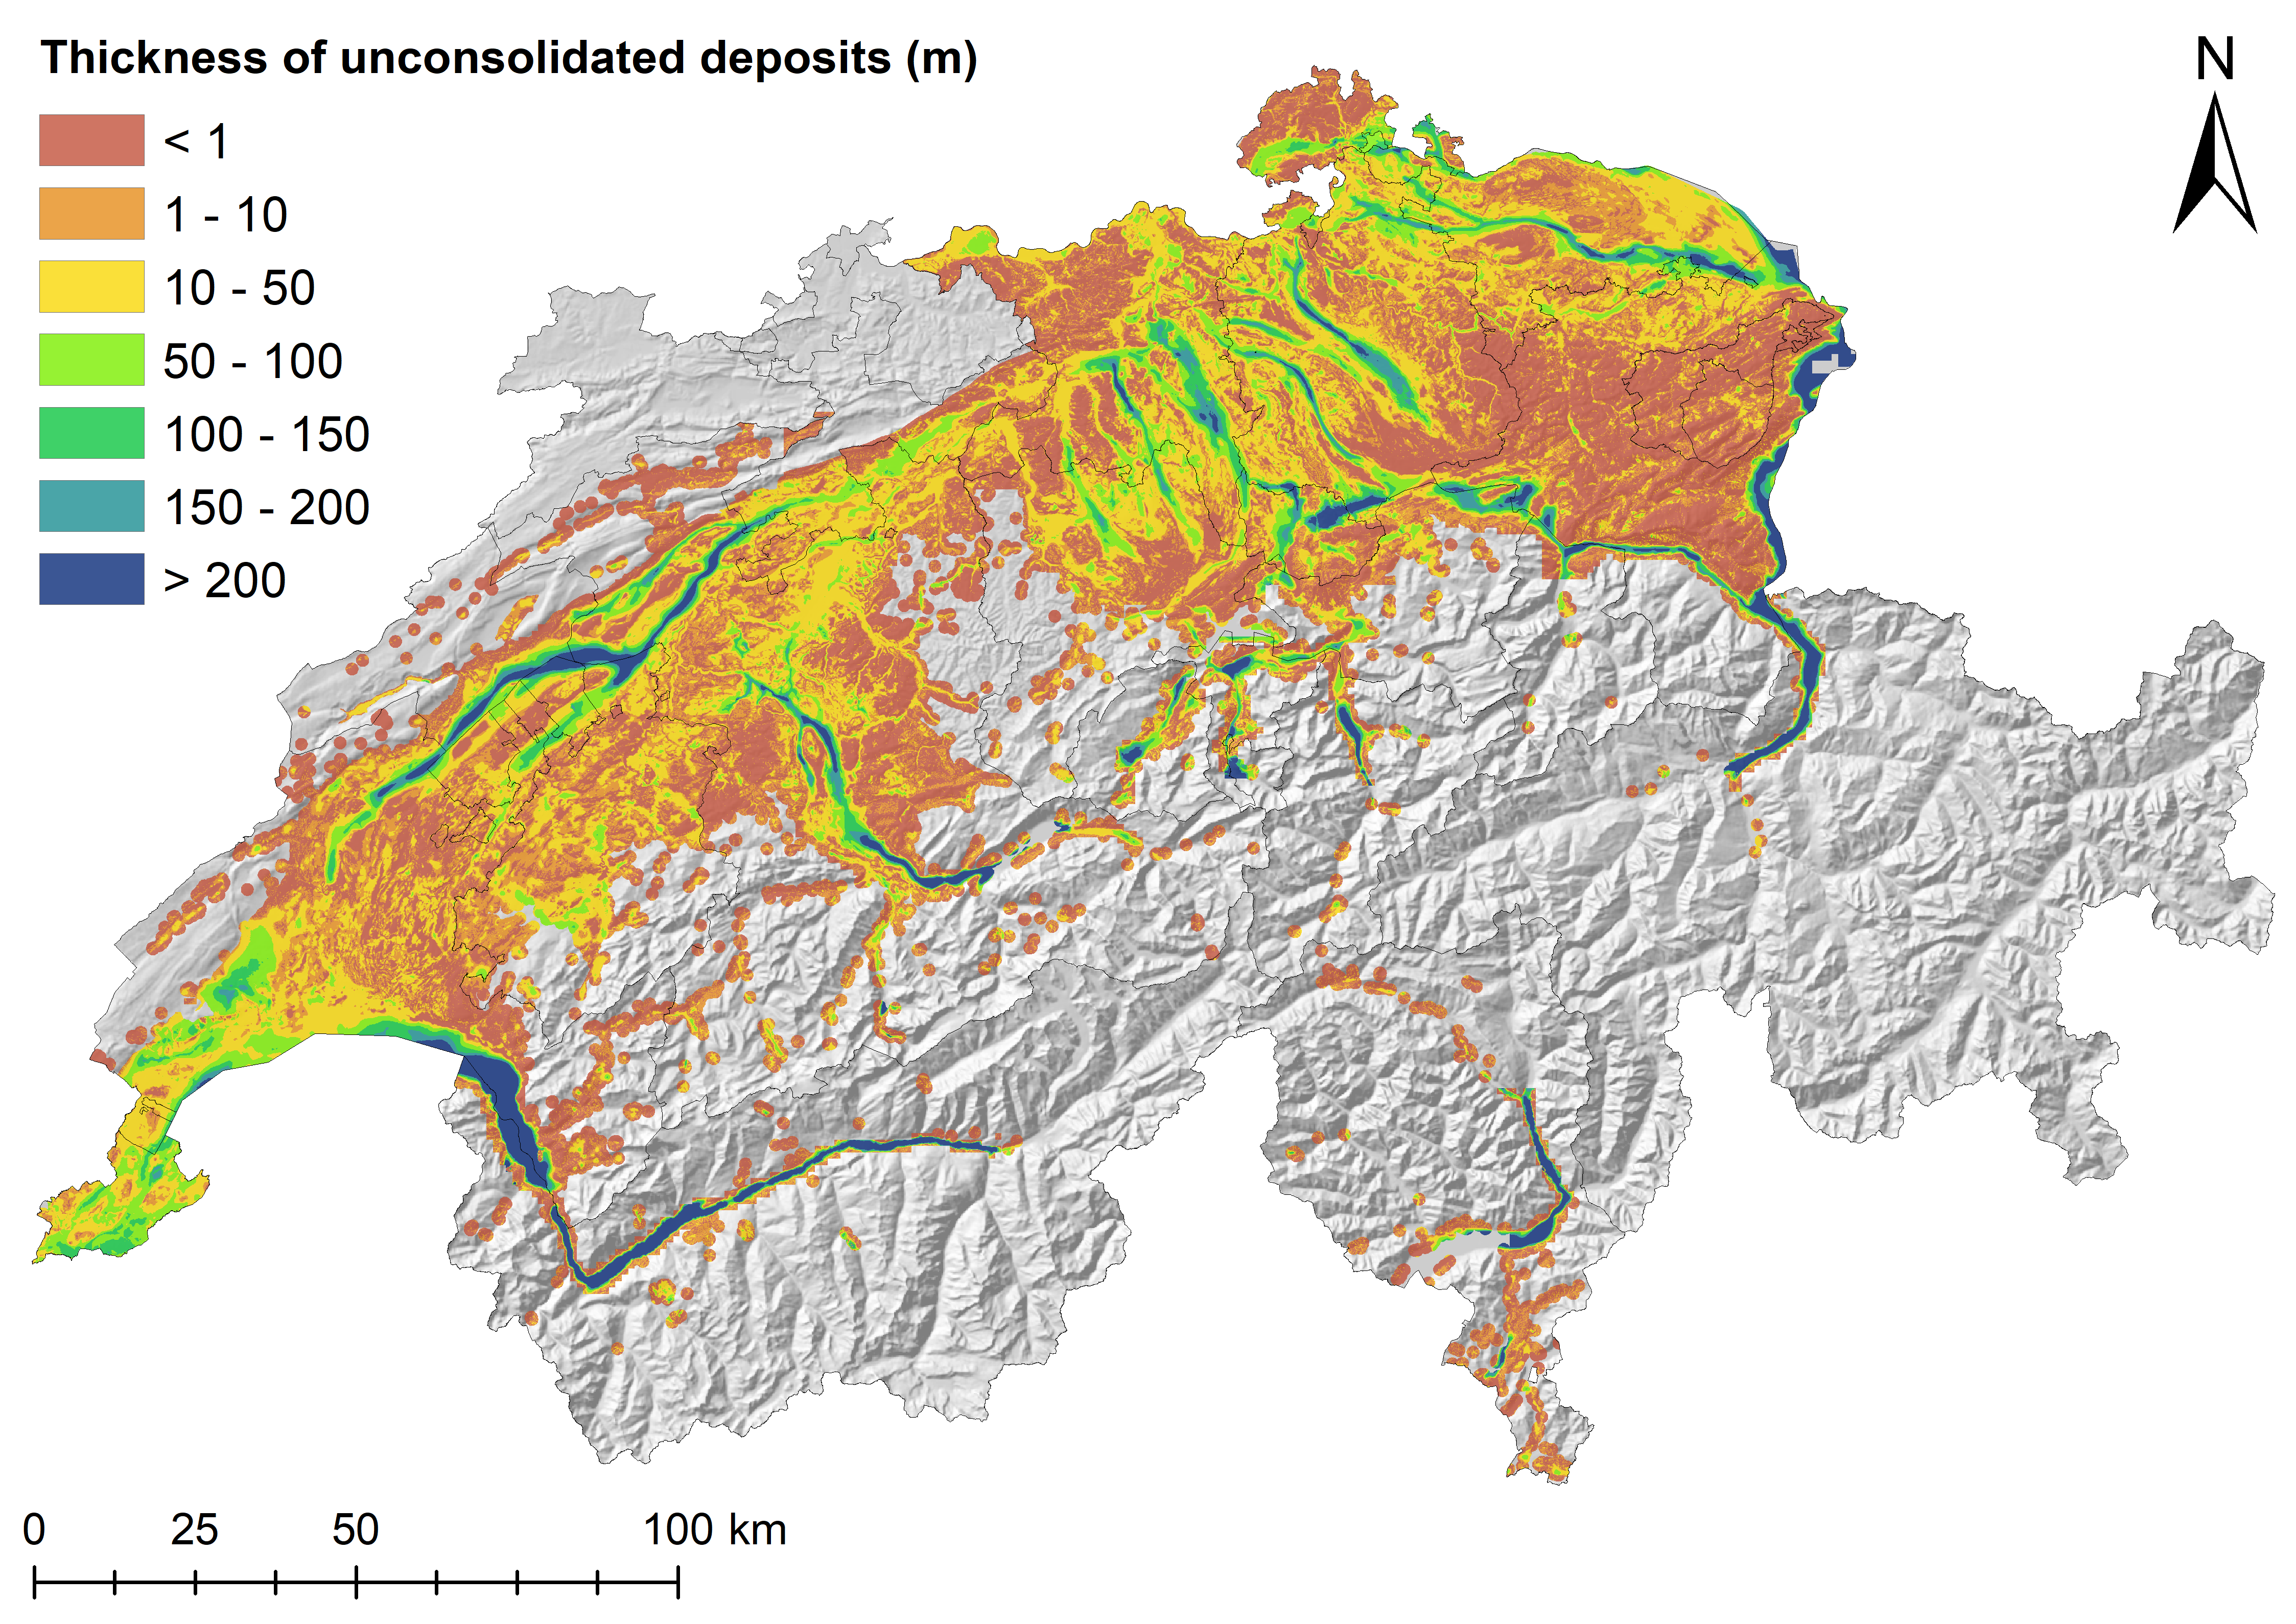
\includegraphics[width=.9\linewidth]{images/Figs/thickness_unconsolidated_deposits_CH.png}  
  \caption{}
  \label{figb:geoCH}
\end{subfigure}
\caption{Geotechnical characteristics of Switzerland. (a) Classification of rock types, and (b) thickness of unconsolidated deposits (in m), available mostly in the Swiss molasse basin and large alluvial plains.}
\label{fig:geoCH}
\end{figure}

\textbf{Geological Maps (GK500).} The GK500 \cite{swisstopo_geomaps_nodate}, published by the Swiss Geological Survey, is a vector dataset of around 13,500 polygons covering the entire Swiss terrain.
The attributes of the polygons contain six primary maps of Switzerland at a scale of 1:500,000, including geological, tectonic and hydrogeological information. 
For the quantification of shallow geothermal potential (Chapter~\ref{geothermal}), the geotechnical maps are the most relevant attributes in the dataset as they allow to map ground thermal properties to the near-surface rock types. 
The GK500 differentiates between four rock types (unconsolidated, sedimentary, magmatic, metamorphous), surface waters and glaciers (see Fig. \ref{figa:geoCH}).
The rock types are further divided into 68 lithology types, which may be aggregated to 26 lithology groups \cite{zappone_saphyr_2021}.

\textbf{Depth of unconsolidated deposits.} 
In addition to the near-surface lithology data provided in the GK500, the depth of the unconsolidated deposits is available from the national geological service (see Fig. \ref{figb:geoCH}). This dataset covers mostly the Swiss Molasse basin (spanning from the north-east to the south-west of the country) and alluvial plains in large mountain valleys, where the majority of the Swiss population lives. The depth of the unconsolidated deposits may be used to improve the estimate of the thermal ground properties for shallow BHEs by accounting for the near-surface unconsolidated deposits and the underlying (mostly sedimentary) rock.

\subsection{Thermal ground properties}

\textbf{Thermal conductivity ($\mathbf{\lambda}$).} For the Cantons of Vaud and Geneva, high-resolution maps of the thermal conductivity are obtained from the geothermal cadastres \cite{asit_vd_cadastre_2019-1,sitg_cadastre_2019}. 
The data is available for depths of $50-300m$ as pixels of $50m$ spatial resolution in all 3 dimensions.  
The conductivities are computed as the average of the ground properties of each rock layer weighted by % weighted
its thickness, which is given by 3D models of the subsurface \cite{groupe_de_travail_pgg_evaluation_2011-1}.
To obtain a homogeneous dataset for $\lambda$ across both cantons, the polygon data of the geothermal cadastre of Geneva has been converted into raster format of $50 \times 50 \times 50$ m$^3$ in coherence with the cadastre of Vaud.

\textbf{Thermal diffusivity ($\mathbf{\alpha}$).}
The thermal diffusivity is obtained from maps of the heat capacity ($\rho C$) as $\alpha = \lambda / \rho C$ (see Eq.~\ref{eq:alpha}). 
Heat capacity data is available only in the Canton of Geneva.
To obtain $\alpha$ for both geothermal cadastres, missing values for $\rho C$ have been estimated as weighted averages using
tabulated data \cite{groupe_de_travail_pgg_evaluation_2011-1, sia_sondes_2010}, and Eq.~\ref{eq:alpha} has been applied to the rasterised maps of $\rho C$ using the same spatial resolution as the thermal conductivity.

%To obtain $\lambda$ and $\rho C$ for all scenarios of $H$ in the entire study region, we compute any missing values as weighted averages using
%tabulated data \cite{groupe_de_travail_pgg_evaluation_2011-1, sia_sondes_2010}. 

\textbf{Ground surface temperature.}
The ground surface temperature ($T_0$) has been provided by \citet{assouline_machine_2019} for pixels of $200 \times 200$ m$^2$ resolution.
The data is estimated from ground measurements using Machine Learning \cite{assouline_machine_2019}.
To minimise the impact of the built environment on these measurements, we use the annual average ground temperature at a depth of 1m.
Its interpolated values at the resolution of $\lambda$ and $\alpha$ is shown in Fig.~\ref{fig:T0}.
To obtain the ground temperature at typical borehole depths, $T_0$ is combined with the temperature gradient in the Swiss plateau, which is approximately constant at 0.03 K/m \cite{sia_sondes_2010} (see Chapter~\ref{geo_params}).

\begin{figure}[tb]
\centering
  % include second image
  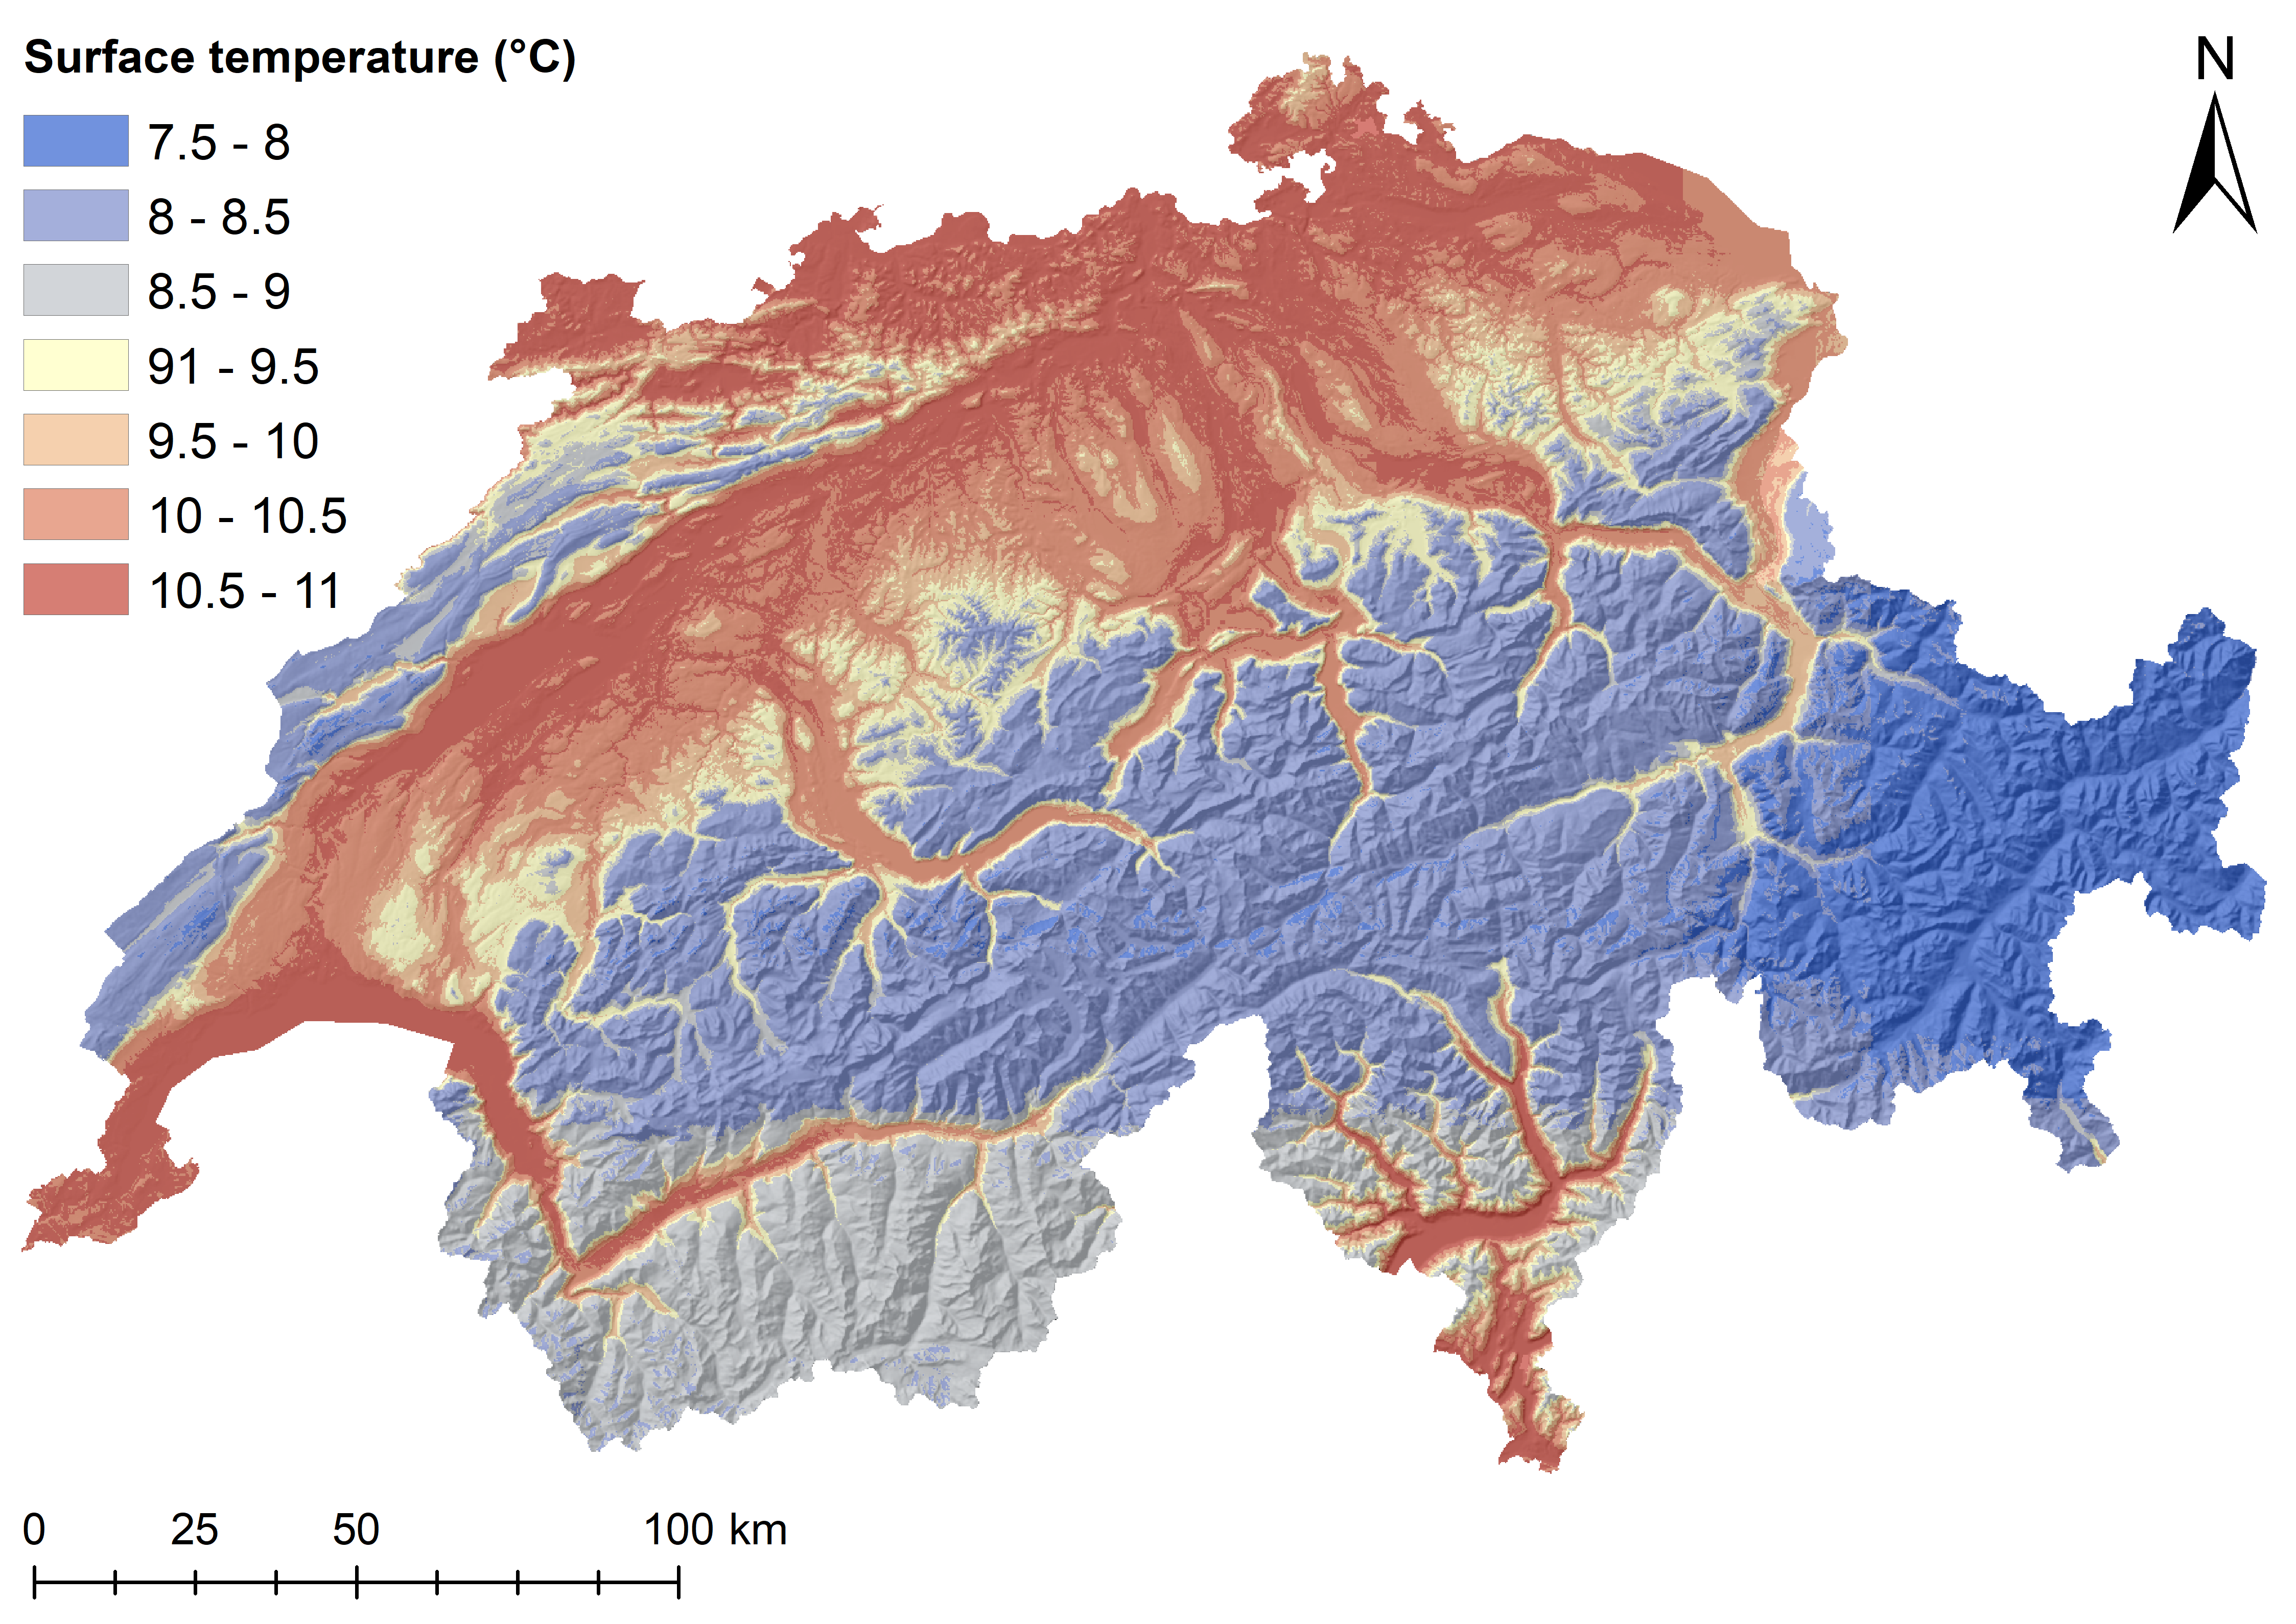
\includegraphics[width=.7\linewidth]{images/Figs/T_surface_CH.png}  
\caption{Ground surface temperatue ($T_0$) at 1m depth for Switzerland \cite{assouline_machine_2019}.}
\label{fig:T0_CH}
\end{figure}

\begin{comment}
\textbf{Geothermal heat flow.}  A map of geothermal heat flows in Switzerland is shown in Fig.~\ref{fig:q_geo}. It was created by Medici and Rybach in 1995 and updated by Sachs and Eberhard in 2010\footnote{Available at: \url{https://opendata.swiss/de/dataset/geothermische-karte-der-schweiz-1-500000}}. As this map was generated by interpolating the measurements from few drilling points, concentrated primarily in the molasse basin, 
--> THIS DATA WAS GENERATED FROM THE TEMPERATURE GRADIENT AND LAMBDA, NOT FROM ACTUAL MEASUREMENTS (SEE LINK!!) - it is currently being updated

\begin{subfigure}{.49\textwidth}
  \centering
  % include first image
  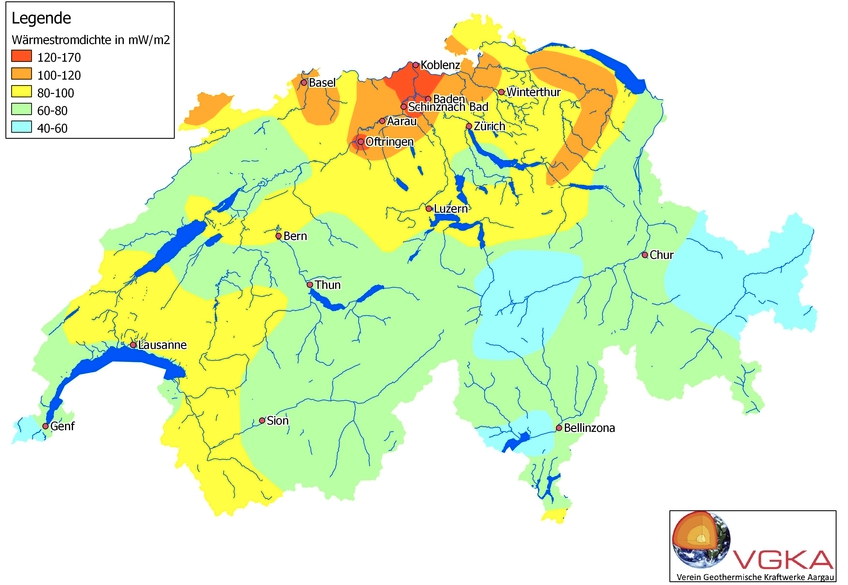
\includegraphics[width=.9\linewidth]{images/Figs/q_geo.png}  
  \caption{}
  \label{fig:q_geo}
\end{subfigure}
\end{comment}

\subsection{Restrictions for geothermal installations [\textit{TO BE DEFINED FOR CH}]}

\textbf{Restriction zones.}
The restriction zones as indicated in the geothermal cadastres \cite{asit_vd_cadastre_2019-1,sitg_cadastre_2019} are divided into three categories, which indicate whether the installation of BHEs is permitted, limited, or prohibited.
Prohibited zones are excluded from this work. 
As no data on the allowed drilling depth is available, the depth of existing installations, obtained from parsing a dataset of existing BHEs, is used in Chapter~\ref{case_study} to approximate a maximum allowed drilling depth.
% The permitted and limited zones are overlaid with information from existing installations to derive the maximum allowed borehole depth ($H_{max}$), 
% Based on these considerations, we choose $H_{max}$ as the $75^{th}$ percentile of the depth of the existing BHEs, yielding values of $200m$ and $150m$ for the "permitted" and "limited" zones, respectively. 